\section{Introduction}
\label{sec:introduction}

\PARstart{A}{fter} a load is restored or a line is reclosed, the machines
continue moving. A second intervention may begin before that response has
decayed. With only eight PMUs in a 39-bus network, a change in a measured
signal may therefore indicate a new source, recovery from an earlier source,
or an imperfect physical prediction. The task is to distinguish these
explanations using only the reports available at the decision time.

\begin{figure*}[t]\centering
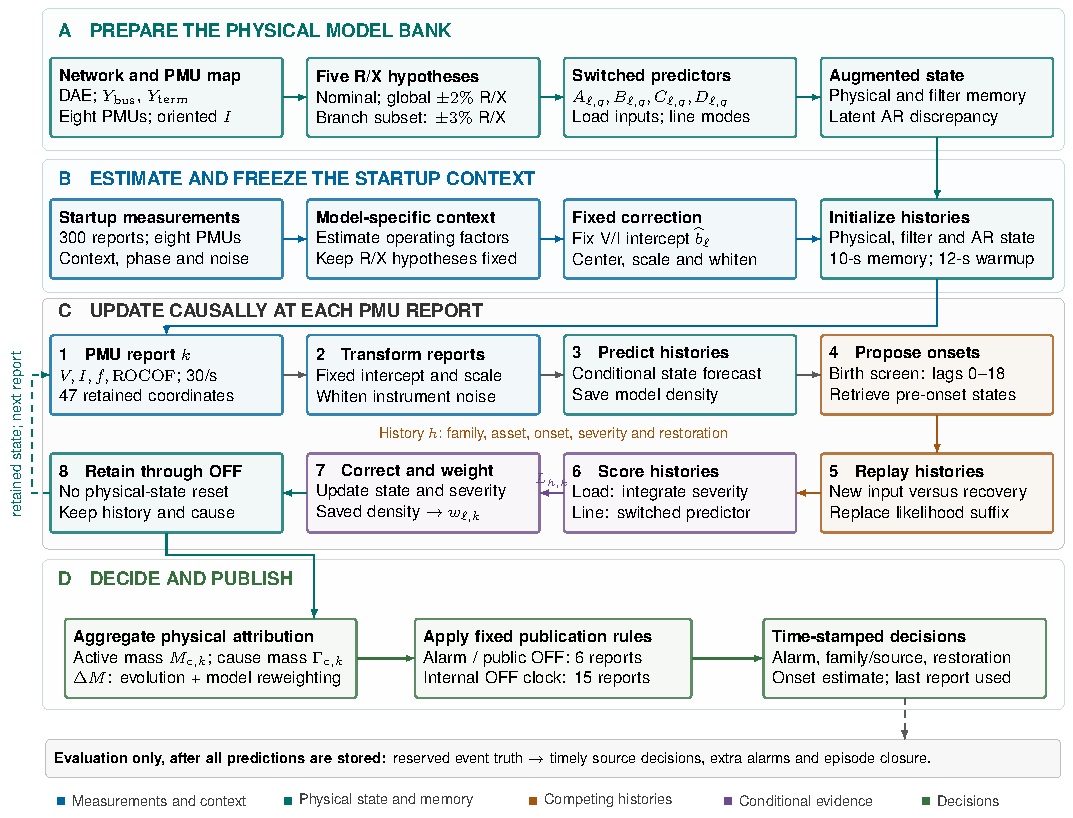
\includegraphics[width=.98\textwidth]{figures/generated/narrative_architecture.pdf}
\caption{Implemented physical inference in four stages. (A) Construct switched network and PMU predictors. (B) Estimate the startup context and fix its observation correction. (C) Compare new intervention histories with retained recovery at each report, using stored pre-onset states. (D) Aggregate attribution and publish qualified alarm, source and restoration decisions. The public six-report rules and the internal 15-report OFF clock are distinct; their support conditions are specified in Section~\ref{sec:narrative-method}. Dashed feedback retains state for the next report. Reserved truth enters only the later evaluation.}
\label{fig:joint-architecture}\end{figure*}

Physical restoration does not erase machine motion. A flat reference can
mislabel its remaining oscillation as a second event; suppressing all alarms
during recovery can hide an actual second event. A corrected voltage offset
also need not correct the response to a later input.

DAE estimators recover unmeasured electrical states
\cite{katanic2024recursive}; outage detectors compare physical hypotheses
\cite{chen2016quickest,rovatsos2017outage}; and simulated trajectories
support sparse-PMU fault diagnosis \cite{warner2023highfidelity}. These
ingredients are established. Our question is whether a continuing recovery
should explain a new PMU change or yield to a later intervention hypothesis.

We test a bank of physical histories, each with a source, onset, severity
and possible restoration. A retained state predicts recovery; a new history
starts from that same estimated state. The contribution is the specified
competition and publication procedure for successive load and line events,
together with a sealed comparison that reports correct attribution and alarm
cost. The comparison retains the feature-based route developed after our
hackathon submission: causal statistics of voltage, current, frequency and
ROCOF feed frozen ExtraTrees models. Thus the paper tests an explicit choice:
does predicting each possible intervention from the electrical model recover
sources missed by a learned summary of the same PMU history, and at what
alarm cost? In that comparison the physical bank attributes
\ReaderPhysicalLoad{}/\ReaderFamilyTotal{} load realizations before OFF
versus \ReaderETLoad{}/\ReaderFamilyTotal{} for the frozen ExtraTrees
reference, but raises \ReaderPhysicalOutsideExtras{} versus
\ReaderETOutsideExtras{} unmatched alarms under out-of-bank R/X. Recovery
memory is part of the procedure; its isolated contribution to that
performance remains unmeasured. The original hackathon model and its
historical metrics are described separately because its 30-s windows and
event catalog differ from this causal test.

The test uses nine candidate load buses and nine lines in a fixed IEEE-39
simulation. It does not establish an all-family hackathon score, calibrated
event probabilities or real-time deployment.
